% Options for packages loaded elsewhere
\PassOptionsToPackage{unicode}{hyperref}
\PassOptionsToPackage{hyphens}{url}
%
\documentclass[
]{article}
\usepackage{amsmath,amssymb}
\usepackage{iftex}
\ifPDFTeX
  \usepackage[T1]{fontenc}
  \usepackage[utf8]{inputenc}
  \usepackage{textcomp} % provide euro and other symbols
\else % if luatex or xetex
  \usepackage{unicode-math} % this also loads fontspec
  \defaultfontfeatures{Scale=MatchLowercase}
  \defaultfontfeatures[\rmfamily]{Ligatures=TeX,Scale=1}
\fi
\usepackage{lmodern}
\ifPDFTeX\else
  % xetex/luatex font selection
\fi
% Use upquote if available, for straight quotes in verbatim environments
\IfFileExists{upquote.sty}{\usepackage{upquote}}{}
\IfFileExists{microtype.sty}{% use microtype if available
  \usepackage[]{microtype}
  \UseMicrotypeSet[protrusion]{basicmath} % disable protrusion for tt fonts
}{}
\makeatletter
\@ifundefined{KOMAClassName}{% if non-KOMA class
  \IfFileExists{parskip.sty}{%
    \usepackage{parskip}
  }{% else
    \setlength{\parindent}{0pt}
    \setlength{\parskip}{6pt plus 2pt minus 1pt}}
}{% if KOMA class
  \KOMAoptions{parskip=half}}
\makeatother
\usepackage{xcolor}
\usepackage[margin=1in]{geometry}
\usepackage{color}
\usepackage{fancyvrb}
\newcommand{\VerbBar}{|}
\newcommand{\VERB}{\Verb[commandchars=\\\{\}]}
\DefineVerbatimEnvironment{Highlighting}{Verbatim}{commandchars=\\\{\}}
% Add ',fontsize=\small' for more characters per line
\usepackage{framed}
\definecolor{shadecolor}{RGB}{248,248,248}
\newenvironment{Shaded}{\begin{snugshade}}{\end{snugshade}}
\newcommand{\AlertTok}[1]{\textcolor[rgb]{0.94,0.16,0.16}{#1}}
\newcommand{\AnnotationTok}[1]{\textcolor[rgb]{0.56,0.35,0.01}{\textbf{\textit{#1}}}}
\newcommand{\AttributeTok}[1]{\textcolor[rgb]{0.13,0.29,0.53}{#1}}
\newcommand{\BaseNTok}[1]{\textcolor[rgb]{0.00,0.00,0.81}{#1}}
\newcommand{\BuiltInTok}[1]{#1}
\newcommand{\CharTok}[1]{\textcolor[rgb]{0.31,0.60,0.02}{#1}}
\newcommand{\CommentTok}[1]{\textcolor[rgb]{0.56,0.35,0.01}{\textit{#1}}}
\newcommand{\CommentVarTok}[1]{\textcolor[rgb]{0.56,0.35,0.01}{\textbf{\textit{#1}}}}
\newcommand{\ConstantTok}[1]{\textcolor[rgb]{0.56,0.35,0.01}{#1}}
\newcommand{\ControlFlowTok}[1]{\textcolor[rgb]{0.13,0.29,0.53}{\textbf{#1}}}
\newcommand{\DataTypeTok}[1]{\textcolor[rgb]{0.13,0.29,0.53}{#1}}
\newcommand{\DecValTok}[1]{\textcolor[rgb]{0.00,0.00,0.81}{#1}}
\newcommand{\DocumentationTok}[1]{\textcolor[rgb]{0.56,0.35,0.01}{\textbf{\textit{#1}}}}
\newcommand{\ErrorTok}[1]{\textcolor[rgb]{0.64,0.00,0.00}{\textbf{#1}}}
\newcommand{\ExtensionTok}[1]{#1}
\newcommand{\FloatTok}[1]{\textcolor[rgb]{0.00,0.00,0.81}{#1}}
\newcommand{\FunctionTok}[1]{\textcolor[rgb]{0.13,0.29,0.53}{\textbf{#1}}}
\newcommand{\ImportTok}[1]{#1}
\newcommand{\InformationTok}[1]{\textcolor[rgb]{0.56,0.35,0.01}{\textbf{\textit{#1}}}}
\newcommand{\KeywordTok}[1]{\textcolor[rgb]{0.13,0.29,0.53}{\textbf{#1}}}
\newcommand{\NormalTok}[1]{#1}
\newcommand{\OperatorTok}[1]{\textcolor[rgb]{0.81,0.36,0.00}{\textbf{#1}}}
\newcommand{\OtherTok}[1]{\textcolor[rgb]{0.56,0.35,0.01}{#1}}
\newcommand{\PreprocessorTok}[1]{\textcolor[rgb]{0.56,0.35,0.01}{\textit{#1}}}
\newcommand{\RegionMarkerTok}[1]{#1}
\newcommand{\SpecialCharTok}[1]{\textcolor[rgb]{0.81,0.36,0.00}{\textbf{#1}}}
\newcommand{\SpecialStringTok}[1]{\textcolor[rgb]{0.31,0.60,0.02}{#1}}
\newcommand{\StringTok}[1]{\textcolor[rgb]{0.31,0.60,0.02}{#1}}
\newcommand{\VariableTok}[1]{\textcolor[rgb]{0.00,0.00,0.00}{#1}}
\newcommand{\VerbatimStringTok}[1]{\textcolor[rgb]{0.31,0.60,0.02}{#1}}
\newcommand{\WarningTok}[1]{\textcolor[rgb]{0.56,0.35,0.01}{\textbf{\textit{#1}}}}
\usepackage{graphicx}
\makeatletter
\def\maxwidth{\ifdim\Gin@nat@width>\linewidth\linewidth\else\Gin@nat@width\fi}
\def\maxheight{\ifdim\Gin@nat@height>\textheight\textheight\else\Gin@nat@height\fi}
\makeatother
% Scale images if necessary, so that they will not overflow the page
% margins by default, and it is still possible to overwrite the defaults
% using explicit options in \includegraphics[width, height, ...]{}
\setkeys{Gin}{width=\maxwidth,height=\maxheight,keepaspectratio}
% Set default figure placement to htbp
\makeatletter
\def\fps@figure{htbp}
\makeatother
\setlength{\emergencystretch}{3em} % prevent overfull lines
\providecommand{\tightlist}{%
  \setlength{\itemsep}{0pt}\setlength{\parskip}{0pt}}
\setcounter{secnumdepth}{5}
\usepackage{fvextra}
\DefineVerbatimEnvironment{Highlighting}{Verbatim}{breaklines=true,breakanywhere=true,commandchars=\\\{\}}
\ifLuaTeX
  \usepackage{selnolig}  % disable illegal ligatures
\fi
\usepackage{bookmark}
\IfFileExists{xurl.sty}{\usepackage{xurl}}{} % add URL line breaks if available
\urlstyle{same}
\hypersetup{
  pdftitle={The Effect of Soil Moisture Content on the Growth and Hexadecane Remediation Capacity of },
  pdfauthor={Y3948024},
  hidelinks,
  pdfcreator={LaTeX via pandoc}}

\title{The Effect of Soil Moisture Content on the Growth and Hexadecane
Remediation Capacity of \emph{Pseudomonas putida}}
\author{Y3948024}
\date{03 May 2025}

\begin{document}
\maketitle

\section{Experimental overview}\label{experimental-overview}

This study investigated how moisture level in the growth media affects
the proliferation of saprophytic bacterium \emph{Pseudomonas putida} and
its ability to degrade hexadecane, a common hydrocarbon pollutant. We
aim to advise on efficacy of \emph{P. putida} to clean oil spills in
environments with different aridity and humidity, such as the 2024 Libya
pipe burst (Rédaction Africanews, 2024) and the recent spills in the
Ecuadorian Amazon (Shanna Hanbury, 2025).

Bacterial growth was quantified using colony-forming unit (CFU) counts
from spot plates prepared via serial dilution of the soil suspended in
\(\frac{1}{4}\) strength Ringer solution (Ringer, 1883). 4 replicates
were used per spot plate, with 3 plates per sample.

The identity of the bacteria was confirmed by a series of tests,
including oxidase testing, light microscopy, culturing on selective
media, and PCR followed by gel electrophoresis.

\subsection{Description of data}\label{description-of-data}

Mean colony counts were normalised to CFU per gram of dry soil. Relevant
datasets include:

\begin{itemize}
\tightlist
\item
  General data: \texttt{cfu\_per\_g\_d\_soil\_allgroups.xlsx}
\item
  Group 3 (spot replicate) data:
  \texttt{cfu\_per\_g\_d\_soil\_group3.xlsx}
\item
  Pre-incubation values: Sheet 4 in the general dataset
\item
  Gel image (PCR): \texttt{data\_gel\_image}
\end{itemize}

Data files are stored under the directory:
\texttt{/Y3948024/analysis/data}. This is required for the .rmd to knit
successfully.

\subsection{Analytical Overview}\label{analytical-overview}

All data processing and visualisation were conducted in \textbf{R
version 4.4.1 (2024-06-14) -- ``Race for Your Life''} via
\textbf{RStudio}, using \textbf{Git} for version control on macOS
Sequoia (v15.3.1).

\subsubsection{Tests used:}\label{tests-used}

\begin{itemize}
\tightlist
\item
  \textbf{Normality}: Shapiro--Wilk test (Shapiro \& Wilk, 1965)
\item
  \textbf{Variance homogeneity}: Levene's test (Levene, 1960)
\item
  \textbf{Non-parametric comparison}: Scheirer--Ray--Hare test (Scheirer
  et al., 1976)
\item
  \textbf{Post-hoc pairwise comparison} Dunn's test (Dunn, 1964)
\end{itemize}

\subsubsection{Packages and Software}\label{packages-and-software}

All packages were obtained from CRAN (Accessed 14 April 2025). Citations
for each package are included inline using standard references.

\begin{itemize}
\tightlist
\item
  \textbf{\texttt{tidyverse}} (Wickham et al., 2019)
\item
  \textbf{\texttt{ggplot2}} (Wickham, 2016)
\item
  \textbf{\texttt{FSA}} (Ogle et al., 2024)
\item
  \textbf{\texttt{readxl}} (Wickham and Bryan, 2023)
\item
  \textbf{\texttt{scales}} (Wickham and Seidel, 2022)
\item
  \textbf{\texttt{vegan}} (Oksanen et al., 2022)
\item
  \textbf{\texttt{rcompanion}} (Mangiafico, 2024)
\item
  \textbf{\texttt{ggpubr}} (Kassambara, 2023)
\item
  \textbf{\texttt{car}} (Fox and Weisberg, 2019)
\end{itemize}

\subsection{Note}\label{note}

Bonferroni correction was used to test for differences in mean CFU count
between contaminated and uncontaminated samples, while
Benjamini-Hochberg correction was used to test for differences between
soil moisture levels. This is because, in the former case, we were only
testing between two groups; in the latter, we were testing 6 pairwise
comparisons across 4 groups, which would inflate the type I error rate.
Thus, we used the more powerful BH correction to increase sensitivity
while still controlling the false discovery rate. The results of the
Dunn's test were not consistent across the two corrections, so the
results should be considered with caution.

\section{Load required libraries}\label{load-required-libraries}

\begin{Shaded}
\begin{Highlighting}[]
\FunctionTok{library}\NormalTok{(tidyverse)      }\CommentTok{\# data manipulation + wrangling (Wickham et al., 2019)}
\FunctionTok{library}\NormalTok{(ggplot2)        }\CommentTok{\# data visualisation (Wickham, 2016)}
\FunctionTok{library}\NormalTok{(FSA)            }\CommentTok{\# non{-}parametric testing (Ogle et al., 2024)}
\FunctionTok{library}\NormalTok{(readxl)         }\CommentTok{\# read Excel files (Wickham and Bryan, 2023)}
\FunctionTok{library}\NormalTok{(scales)         }\CommentTok{\# scale customisation for plots (Wickham and Seidel, 2022)}
\FunctionTok{library}\NormalTok{(vegan)          }\CommentTok{\# multivariate ecology tools (Oksanen et al., 2022)}
\FunctionTok{library}\NormalTok{(rcompanion)     }\CommentTok{\# statistics for extension work (Mangiafico, 2024)}
\FunctionTok{library}\NormalTok{(ggpubr)         }\CommentTok{\# ggplot2 enhancements (Kassambara, 2023)}
\FunctionTok{library}\NormalTok{(car)            }\CommentTok{\# regression diagnostics (Fox and Weisberg, 2019)}
\end{Highlighting}
\end{Shaded}

\section{Statistical analysis and visualisation of data from plate
replicates}\label{statistical-analysis-and-visualisation-of-data-from-plate-replicates}

\subsection{Read in all Excel sheets and add a new column indicating the
group each row came
from}\label{read-in-all-excel-sheets-and-add-a-new-column-indicating-the-group-each-row-came-from}

\begin{Shaded}
\begin{Highlighting}[]
\NormalTok{path }\OtherTok{\textless{}{-}} \StringTok{\textquotesingle{}data/cfu\_per\_g\_d\_soil\_allgroups.xlsx\textquotesingle{}}
\NormalTok{data\_allgroups }\OtherTok{\textless{}{-}} \FunctionTok{excel\_sheets}\NormalTok{(path)}
\NormalTok{data\_tidy\_list }\OtherTok{\textless{}{-}} \FunctionTok{lapply}\NormalTok{(data\_allgroups, }\ControlFlowTok{function}\NormalTok{(sheet) \{}
\NormalTok{  data }\OtherTok{\textless{}{-}} \FunctionTok{read\_excel}\NormalTok{(path, }\AttributeTok{sheet =}\NormalTok{ sheet)  }\CommentTok{\# read each sheet}
\NormalTok{  data}\SpecialCharTok{$}\NormalTok{group }\OtherTok{\textless{}{-}}\NormalTok{ sheet                      }\CommentTok{\# tag with group label}
  \FunctionTok{return}\NormalTok{(data)}
\NormalTok{\})}
\end{Highlighting}
\end{Shaded}

\subsection{Combine all data into a single data frame and coerce
variables to
factors}\label{combine-all-data-into-a-single-data-frame-and-coerce-variables-to-factors}

\begin{Shaded}
\begin{Highlighting}[]
\NormalTok{data\_tidy }\OtherTok{\textless{}{-}} \FunctionTok{do.call}\NormalTok{(rbind, data\_tidy\_list)}
\NormalTok{data\_tidy}\SpecialCharTok{$}\NormalTok{plate }\OtherTok{\textless{}{-}} \FunctionTok{as.factor}\NormalTok{(data\_tidy}\SpecialCharTok{$}\NormalTok{plate)}
\NormalTok{data\_tidy}\SpecialCharTok{$}\NormalTok{Contamination }\OtherTok{\textless{}{-}} \FunctionTok{as.factor}\NormalTok{(data\_tidy}\SpecialCharTok{$}\NormalTok{Contamination)}
\NormalTok{data\_tidy}\SpecialCharTok{$}\NormalTok{group }\OtherTok{\textless{}{-}} \FunctionTok{as.factor}\NormalTok{(data\_tidy}\SpecialCharTok{$}\NormalTok{group)}
\end{Highlighting}
\end{Shaded}

\subsection{Summarise data}\label{summarise-data}

Calculate means, standard deviation, sample size and standard error

\begin{Shaded}
\begin{Highlighting}[]
\CommentTok{\# Exclude pre{-}incubation data (group 4)}
\NormalTok{data\_summary }\OtherTok{\textless{}{-}}\NormalTok{ data\_tidy }\SpecialCharTok{\%\textgreater{}\%}
  \FunctionTok{filter}\NormalTok{(group }\SpecialCharTok{!=} \StringTok{"4"}\NormalTok{) }\SpecialCharTok{\%\textgreater{}\%}
  \FunctionTok{group\_by}\NormalTok{(plate, Contamination) }\SpecialCharTok{\%\textgreater{}\%}
  \FunctionTok{summarise}\NormalTok{(}\AttributeTok{mean =} \FunctionTok{mean}\NormalTok{(cfu\_count),}
            \AttributeTok{sd =} \FunctionTok{sd}\NormalTok{(cfu\_count),}
            \AttributeTok{n =} \FunctionTok{n}\NormalTok{(),}
            \AttributeTok{se =}\NormalTok{ sd }\SpecialCharTok{/} \FunctionTok{sqrt}\NormalTok{(n))}
\end{Highlighting}
\end{Shaded}

\begin{Shaded}
\begin{Highlighting}[]
\NormalTok{data\_summary}
\end{Highlighting}
\end{Shaded}

\begin{verbatim}
## # A tibble: 8 x 6
## # Groups:   plate [4]
##   plate Contamination             mean          sd     n          se
##   <fct> <fct>                    <dbl>       <dbl> <int>       <dbl>
## 1 30    With hexadecane     352887896.  357877255.     3  206620530.
## 2 30    Without hexadecane   48226222.   43478923.     3   25102568.
## 3 40    With hexadecane    2645521618. 4348823641.     3 2510794500.
## 4 40    Without hexadecane   86096111.   42394654.     3   24476565.
## 5 50    With hexadecane    1224751382. 1547511269.     3  893456048.
## 6 50    Without hexadecane  338414694.  368077310.     3  212509534.
## 7 60    With hexadecane     505089743.  661967720.     3  382187241.
## 8 60    Without hexadecane  388161944.  495927219.     3  286323713.
\end{verbatim}

\subsection{Statistical tests}\label{statistical-tests}

\subsubsection{Fit a linear model on CFU count by moisture level and
contamination
status}\label{fit-a-linear-model-on-cfu-count-by-moisture-level-and-contamination-status}

\begin{Shaded}
\begin{Highlighting}[]
\NormalTok{mod }\OtherTok{\textless{}{-}} \FunctionTok{lm}\NormalTok{(cfu\_count }\SpecialCharTok{\textasciitilde{}}\NormalTok{ plate }\SpecialCharTok{+}\NormalTok{ Contamination, }\AttributeTok{data =}\NormalTok{ data\_tidy }\SpecialCharTok{\%\textgreater{}\%} \FunctionTok{filter}\NormalTok{(group }\SpecialCharTok{!=} \StringTok{"4"}\NormalTok{))}
\end{Highlighting}
\end{Shaded}

\subsubsection{Use the Freedman-Diaconis rule to determine optimal bin
width for this
histogram}\label{use-the-freedman-diaconis-rule-to-determine-optimal-bin-width-for-this-histogram}

\begin{Shaded}
\begin{Highlighting}[]
\NormalTok{iqr }\OtherTok{\textless{}{-}} \FunctionTok{IQR}\NormalTok{(data\_tidy}\SpecialCharTok{$}\NormalTok{cfu\_count)}
\NormalTok{n }\OtherTok{\textless{}{-}} \FunctionTok{nrow}\NormalTok{(data\_tidy)}
\NormalTok{bin\_width }\OtherTok{\textless{}{-}} \DecValTok{2} \SpecialCharTok{*}\NormalTok{ iqr }\SpecialCharTok{/}\NormalTok{ (n}\SpecialCharTok{\^{}}\NormalTok{(}\DecValTok{1}\SpecialCharTok{/}\DecValTok{3}\NormalTok{))}
\end{Highlighting}
\end{Shaded}

Bin width = 237686445

\subsubsection{Visualise residual distribution to check normality of
residuals}\label{visualise-residual-distribution-to-check-normality-of-residuals}

\begin{Shaded}
\begin{Highlighting}[]
\NormalTok{resid\_df }\OtherTok{\textless{}{-}} \FunctionTok{tibble}\NormalTok{(}\AttributeTok{residuals =}\NormalTok{ mod}\SpecialCharTok{$}\NormalTok{residuals)}
\FunctionTok{ggplot}\NormalTok{(resid\_df, }\FunctionTok{aes}\NormalTok{(}\AttributeTok{x =}\NormalTok{ residuals)) }\SpecialCharTok{+}
  \FunctionTok{geom\_histogram}\NormalTok{(}\AttributeTok{binwidth =}\NormalTok{ bin\_width)}
\end{Highlighting}
\end{Shaded}

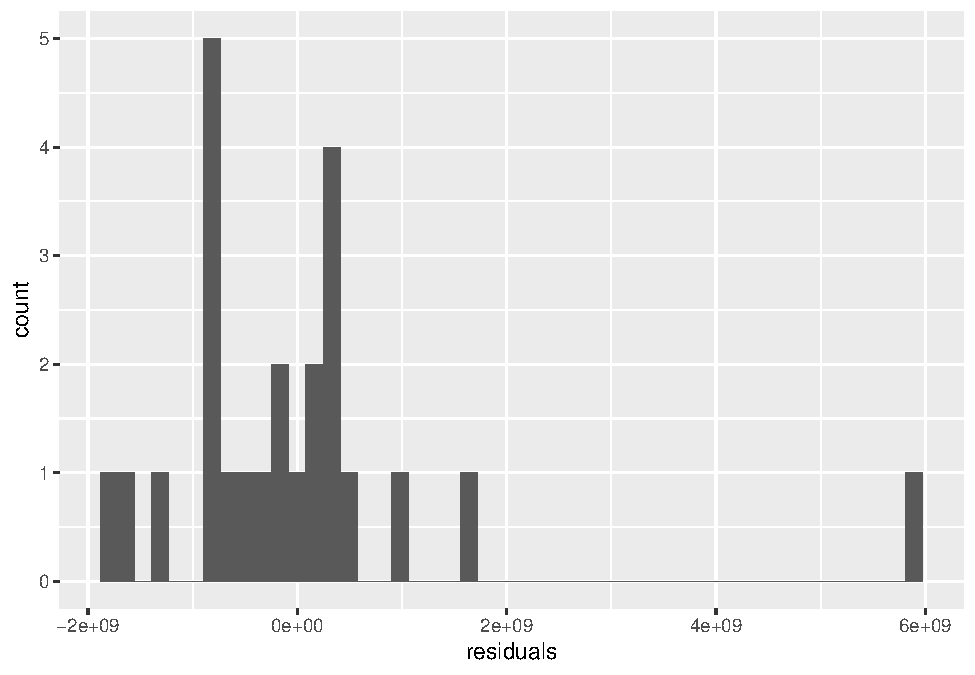
\includegraphics{analysis_files/figure-latex/plot-residuals-allgroups-1.pdf}

The data appears to have a positive skew, with a long tail on the right.
This suggests that the data may not be normally distributed.

\subsubsection{Shapiro-Wilk test for normality of
residuals}\label{shapiro-wilk-test-for-normality-of-residuals}

\begin{Shaded}
\begin{Highlighting}[]
\FunctionTok{shapiro.test}\NormalTok{(mod}\SpecialCharTok{$}\NormalTok{residuals)}
\end{Highlighting}
\end{Shaded}

\begin{verbatim}
## 
##  Shapiro-Wilk normality test
## 
## data:  mod$residuals
## W = 0.73228, p-value = 2.775e-05
\end{verbatim}

p = 2.775e-05 \textless{} 0.05. Therefore there is evidence to suggest
that the residuals are not normally distributed.

\subsubsection{Levene's test for homogeneity of
variance}\label{levenes-test-for-homogeneity-of-variance}

\paragraph{Filter out group 4 (pre-incubation) for homogeneity
testing}\label{filter-out-group-4-pre-incubation-for-homogeneity-testing}

\begin{Shaded}
\begin{Highlighting}[]
\NormalTok{data\_filtered }\OtherTok{\textless{}{-}}\NormalTok{ data\_tidy }\SpecialCharTok{\%\textgreater{}\%} \FunctionTok{filter}\NormalTok{(group }\SpecialCharTok{!=} \StringTok{"4"}\NormalTok{)}
\end{Highlighting}
\end{Shaded}

\paragraph{Fit linear model and conduct Levene's
test}\label{fit-linear-model-and-conduct-levenes-test}

\begin{Shaded}
\begin{Highlighting}[]
\NormalTok{levmod }\OtherTok{\textless{}{-}} \FunctionTok{lm}\NormalTok{(cfu\_count }\SpecialCharTok{\textasciitilde{}}\NormalTok{ plate }\SpecialCharTok{+}\NormalTok{ Contamination, }\AttributeTok{data =}\NormalTok{ data\_filtered)}
\FunctionTok{leveneTest}\NormalTok{(}\FunctionTok{residuals}\NormalTok{(levmod) }\SpecialCharTok{\textasciitilde{}}\NormalTok{ data\_filtered}\SpecialCharTok{$}\NormalTok{group)}
\end{Highlighting}
\end{Shaded}

\begin{verbatim}
## Levene's Test for Homogeneity of Variance (center = median)
##       Df F value Pr(>F)
## group  2  1.3126 0.2903
##       21
\end{verbatim}

p = 0.2903 \textgreater{} 0.05. Therefore, there is not enough evidence
to suggest that the variances are not homogenous across groups.

\paragraph{Plot boxplot of residuals grouped by replicate group to
visualise the spread of
variance}\label{plot-boxplot-of-residuals-grouped-by-replicate-group-to-visualise-the-spread-of-variance}

\begin{Shaded}
\begin{Highlighting}[]
\NormalTok{data\_filtered}\SpecialCharTok{$}\NormalTok{resid }\OtherTok{\textless{}{-}} \FunctionTok{residuals}\NormalTok{(levmod)}
\FunctionTok{ggplot}\NormalTok{(data\_filtered, }\FunctionTok{aes}\NormalTok{(}\AttributeTok{x =}\NormalTok{ group, }\AttributeTok{y =}\NormalTok{ resid)) }\SpecialCharTok{+}
  \FunctionTok{geom\_boxplot}\NormalTok{() }\SpecialCharTok{+}
  \FunctionTok{labs}\NormalTok{(}\AttributeTok{title =} \StringTok{"Residual Variance by Group"}\NormalTok{)}
\end{Highlighting}
\end{Shaded}

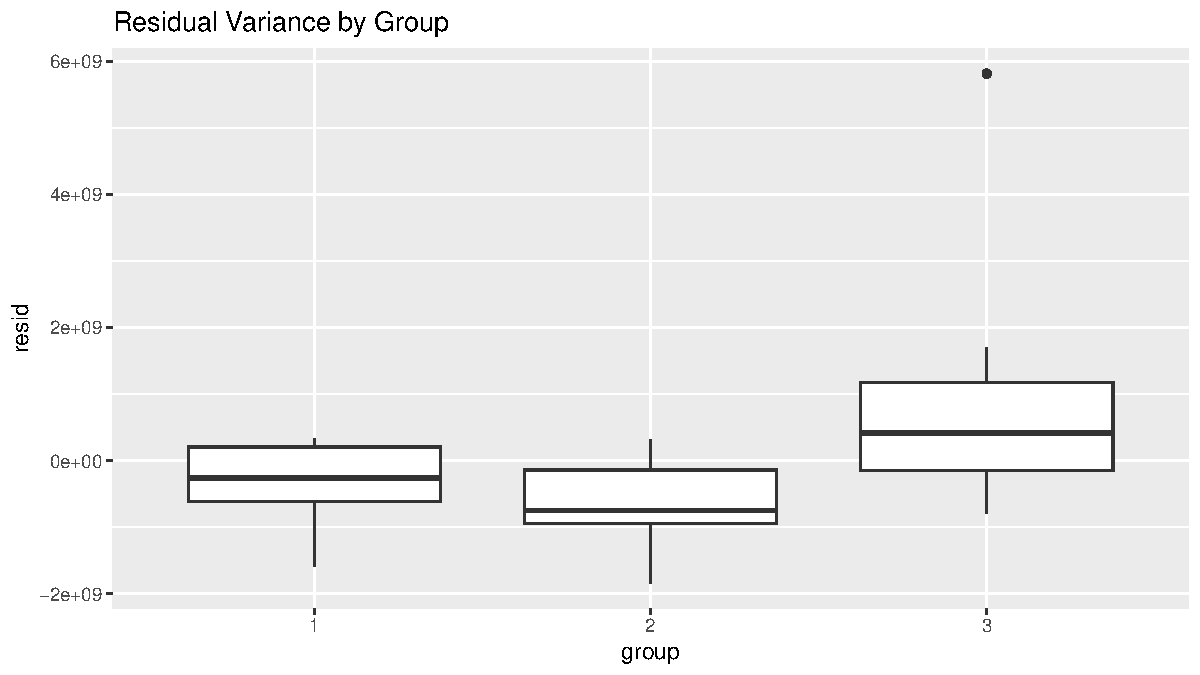
\includegraphics{analysis_files/figure-latex/a-1.pdf}

\subsection{Testing for differences in mean CFU count between soil
moisture levels and contamination
status}\label{testing-for-differences-in-mean-cfu-count-between-soil-moisture-levels-and-contamination-status}

\subsubsection{We will perform a non-parametric test, eg. the
Scheirer-Ray-Hare test, to observe overall
significance}\label{we-will-perform-a-non-parametric-test-eg.-the-scheirer-ray-hare-test-to-observe-overall-significance}

\begin{Shaded}
\begin{Highlighting}[]
\FunctionTok{scheirerRayHare}\NormalTok{(cfu\_count }\SpecialCharTok{\textasciitilde{}}\NormalTok{ plate }\SpecialCharTok{*}\NormalTok{ Contamination, }\AttributeTok{data =} \FunctionTok{filter}\NormalTok{(data\_tidy, group }\SpecialCharTok{!=} \DecValTok{4}\NormalTok{))}
\end{Highlighting}
\end{Shaded}

\begin{verbatim}
## 
## DV:  cfu_count 
## Observations:  24 
## D:  1 
## MS total:  50
\end{verbatim}

\begin{verbatim}
##                     Df Sum Sq      H p.value
## plate                3  98.33 1.9667 0.57935
## Contamination        1  80.67 1.6133 0.20402
## plate:Contamination  3  52.33 1.0467 0.78996
## Residuals           16 918.67
\end{verbatim}

p(Plate:Contamination) = 0.78996 \textgreater{} 0.05, therefore there is
not enough evidence to suggest that soil moisture content affects the
growth of P. putida, using data from all groups.

\subsubsection{Post-hoc pairwise
testing}\label{post-hoc-pairwise-testing}

\paragraph{Post-hoc for Contamination}\label{post-hoc-for-contamination}

\paragraph{}\label{section}

\begin{Shaded}
\begin{Highlighting}[]
\FunctionTok{dunnTest}\NormalTok{(cfu\_count }\SpecialCharTok{\textasciitilde{}}\NormalTok{ Contamination, }\AttributeTok{data =} \FunctionTok{filter}\NormalTok{(data\_tidy, group }\SpecialCharTok{!=} \DecValTok{4}\NormalTok{), }\AttributeTok{method =} \StringTok{"bonferroni"}\NormalTok{)}
\end{Highlighting}
\end{Shaded}

\begin{verbatim}
## Dunn (1964) Kruskal-Wallis multiple comparison
\end{verbatim}

\begin{verbatim}
##   p-values adjusted with the Bonferroni method.
\end{verbatim}

\begin{verbatim}
##                             Comparison        Z   P.unadj     P.adj
## 1 With hexadecane - Without hexadecane 1.270171 0.2040239 0.2040239
\end{verbatim}

p.adj = 0.2040239 \textgreater{} 0.05, therefore there is not enough
evidence to suggest that hexadecane presence does affect growth of P.
putida.

\paragraph{Post-hoc for Plate}\label{post-hoc-for-plate}

\subparagraph{Contamination = With
hexadecane}\label{contamination-with-hexadecane}

\subparagraph{}\label{section-1}

\begin{Shaded}
\begin{Highlighting}[]
\FunctionTok{dunnTest}\NormalTok{(cfu\_count }\SpecialCharTok{\textasciitilde{}}\NormalTok{ plate, }\AttributeTok{data =} \FunctionTok{filter}\NormalTok{(data\_tidy, Contamination }\SpecialCharTok{==} \StringTok{"With hexadecane"}\NormalTok{, group }\SpecialCharTok{!=} \DecValTok{4}\NormalTok{), }\AttributeTok{method =} \StringTok{"bh"}\NormalTok{)}
\end{Highlighting}
\end{Shaded}

\begin{verbatim}
## Dunn (1964) Kruskal-Wallis multiple comparison
\end{verbatim}

\begin{verbatim}
##   p-values adjusted with the Benjamini-Hochberg method.
\end{verbatim}

\begin{verbatim}
##   Comparison          Z P.unadj P.adj
## 1    30 - 40 -0.1132277 0.90985     1
## 2    30 - 50 -0.1132277 0.90985     1
## 3    40 - 50  0.0000000 1.00000     1
## 4    30 - 60  0.0000000 1.00000     1
## 5    40 - 60  0.1132277 0.90985     1
## 6    50 - 60  0.1132277 0.90985     1
\end{verbatim}

\subparagraph{Contamination = Without
hexadecane}\label{contamination-without-hexadecane}

\subparagraph{}\label{section-2}

\begin{Shaded}
\begin{Highlighting}[]
\FunctionTok{dunnTest}\NormalTok{(cfu\_count }\SpecialCharTok{\textasciitilde{}}\NormalTok{ plate, }\AttributeTok{data =} \FunctionTok{filter}\NormalTok{(data\_tidy, Contamination }\SpecialCharTok{==} \StringTok{"Without hexadecane"}\NormalTok{, group }\SpecialCharTok{!=} \DecValTok{4}\NormalTok{), }\AttributeTok{method =} \StringTok{"bh"}\NormalTok{)}
\end{Highlighting}
\end{Shaded}

\begin{verbatim}
## Dunn (1964) Kruskal-Wallis multiple comparison
\end{verbatim}

\begin{verbatim}
##   p-values adjusted with the Benjamini-Hochberg method.
\end{verbatim}

\begin{verbatim}
##   Comparison          Z    P.unadj     P.adj
## 1    30 - 40 -0.5661385 0.57129962 0.6855595
## 2    30 - 50 -1.6984156 0.08942936 0.5365762
## 3    40 - 50 -1.1322770 0.25751798 0.5150360
## 4    30 - 60 -1.5851878 0.11292366 0.3387710
## 5    40 - 60 -1.0190493 0.30817955 0.4622693
## 6    50 - 60  0.1132277 0.90985003 0.9098500
\end{verbatim}

With hexadecane: No significant differences. Without hexadecane: No
significant differences.

Therefore there is not enough evidence to suggest that soil moisture
content affects the growth of P. putida, using meaned data from all 3
groups.

\subsection{Visualise group-level CFU count with mean, SE, and LOESS
lines}\label{visualise-group-level-cfu-count-with-mean-se-and-loess-lines}

\subsubsection{Design a custom theme for the
plot}\label{design-a-custom-theme-for-the-plot}

\begin{Shaded}
\begin{Highlighting}[]
\NormalTok{theme\_custom }\OtherTok{\textless{}{-}} \FunctionTok{theme}\NormalTok{(}
  \AttributeTok{panel.spacing.x =} \FunctionTok{unit}\NormalTok{(}\DecValTok{1}\NormalTok{, }\StringTok{"lines"}\NormalTok{),}
  \AttributeTok{legend.position =} \StringTok{\textquotesingle{}right\textquotesingle{}}\NormalTok{,}
  \AttributeTok{panel.grid.major.y =} \FunctionTok{element\_line}\NormalTok{(}\AttributeTok{colour =} \StringTok{"\#e3e1e1"}\NormalTok{, }\AttributeTok{linetype =} \DecValTok{1}\NormalTok{),}
  \AttributeTok{panel.grid.major.x =} \FunctionTok{element\_line}\NormalTok{(}\AttributeTok{colour =} \StringTok{"\#e3e1e1"}\NormalTok{, }\AttributeTok{linetype =} \DecValTok{1}\NormalTok{),}
  \AttributeTok{panel.grid.minor.y =} \FunctionTok{element\_line}\NormalTok{(}\AttributeTok{colour =} \StringTok{"\#e3e1e1"}\NormalTok{, }\AttributeTok{linetype =} \DecValTok{1}\NormalTok{),}
  \AttributeTok{axis.text.x =} \FunctionTok{element\_text}\NormalTok{(}\AttributeTok{hjust =} \FloatTok{0.5}\NormalTok{),}
  \AttributeTok{plot.title =} \FunctionTok{element\_text}\NormalTok{(}\AttributeTok{size =} \DecValTok{12}\NormalTok{, }\AttributeTok{face =} \StringTok{"bold"}\NormalTok{, }\AttributeTok{hjust =} \FloatTok{0.5}\NormalTok{),}
  \AttributeTok{plot.margin =} \FunctionTok{margin}\NormalTok{(}\DecValTok{10}\NormalTok{, }\DecValTok{10}\NormalTok{, }\DecValTok{10}\NormalTok{, }\DecValTok{10}\NormalTok{),}
  \AttributeTok{plot.subtitle =} \FunctionTok{element\_text}\NormalTok{(}\AttributeTok{vjust =} \SpecialCharTok{{-}}\DecValTok{250}\NormalTok{, }\AttributeTok{hjust =} \DecValTok{1}\NormalTok{)}
\NormalTok{)}
\end{Highlighting}
\end{Shaded}

\subsubsection{Create plot}\label{create-plot}

\begin{Shaded}
\begin{Highlighting}[]
\NormalTok{mean\_CFU\_count }\OtherTok{\textless{}{-}} \FunctionTok{ggplot}\NormalTok{(}\AttributeTok{data =}\NormalTok{ data\_tidy) }\SpecialCharTok{+}
  
  \DocumentationTok{\#\#\#\# Plotting replicate data points}
  \FunctionTok{geom\_point}\NormalTok{(}\FunctionTok{aes}\NormalTok{(}\AttributeTok{x =} \FunctionTok{factor}\NormalTok{(plate), }
                 \AttributeTok{y =}\NormalTok{ cfu\_count, }
                 \AttributeTok{colour =}\NormalTok{ group)) }\SpecialCharTok{+}
  
  \DocumentationTok{\#\#\#\# Plotting LOESS regression lines for replicates from data\_tidy}
  \FunctionTok{geom\_smooth}\NormalTok{(}\FunctionTok{aes}\NormalTok{(}\AttributeTok{x =} \FunctionTok{factor}\NormalTok{(plate), }
                  \AttributeTok{y =}\NormalTok{ cfu\_count, }
                  \AttributeTok{colour =}\NormalTok{ group,}
                  \AttributeTok{group =} \FunctionTok{interaction}\NormalTok{(group, Contamination)), }
              \AttributeTok{method =} \StringTok{"loess"}\NormalTok{, }
              \AttributeTok{se =} \ConstantTok{FALSE}\NormalTok{,}
              \AttributeTok{linewidth =} \FloatTok{0.3}\NormalTok{) }\SpecialCharTok{+}
  
  \DocumentationTok{\#\#\#\# Plotting means from data\_summary}
  \FunctionTok{geom\_point}\NormalTok{(}\AttributeTok{data =}\NormalTok{ data\_summary, }
             \FunctionTok{aes}\NormalTok{(}\AttributeTok{x =} \FunctionTok{factor}\NormalTok{(plate), }
                 \AttributeTok{y =}\NormalTok{ mean), }
             \AttributeTok{colour =} \StringTok{"black"}\NormalTok{, }
             \AttributeTok{size =} \DecValTok{2}\NormalTok{) }\SpecialCharTok{+}
  
  \DocumentationTok{\#\#\#\# Plotting error bars for means from data\_summary}
  \FunctionTok{geom\_errorbar}\NormalTok{(}\AttributeTok{data =}\NormalTok{ data\_summary,}
                \FunctionTok{aes}\NormalTok{(}\AttributeTok{x =} \FunctionTok{factor}\NormalTok{(plate), }
                    \AttributeTok{ymin =}\NormalTok{ mean }\SpecialCharTok{{-}}\NormalTok{ se, }
                    \AttributeTok{ymax =}\NormalTok{ mean }\SpecialCharTok{+}\NormalTok{ se), }
                \AttributeTok{width =} \FloatTok{0.1}\NormalTok{, }
                \AttributeTok{colour =} \StringTok{"black"}\NormalTok{) }\SpecialCharTok{+}
  
  \DocumentationTok{\#\#\#\# Plotting LOESS regression lines for the means}
  \FunctionTok{geom\_smooth}\NormalTok{(}\AttributeTok{data =}\NormalTok{ data\_summary,}
              \FunctionTok{aes}\NormalTok{(}\AttributeTok{x =} \FunctionTok{factor}\NormalTok{(plate), }
                  \AttributeTok{y =}\NormalTok{ mean,}
                  \AttributeTok{group =}\NormalTok{ Contamination), }
              \AttributeTok{method =} \StringTok{"loess"}\NormalTok{, }
              \AttributeTok{colour =} \StringTok{"black"}\NormalTok{,}
              \AttributeTok{se =} \ConstantTok{FALSE}\NormalTok{, }
              \AttributeTok{linewidth =} \DecValTok{1}\NormalTok{) }\SpecialCharTok{+}
  
  \DocumentationTok{\#\#\#\# Adding labels and changing axis}
  \FunctionTok{labs}\NormalTok{(}\AttributeTok{title =} \FunctionTok{expression}\NormalTok{(}\FunctionTok{italic}\NormalTok{(}\StringTok{"Pseudomonas putida"}\NormalTok{)}\SpecialCharTok{\textasciitilde{}}\StringTok{"}\SpecialCharTok{\textbackslash{}n}\StringTok{CFU count per gram of dry soil, by replicate"}\NormalTok{),}
       \AttributeTok{x =} \FunctionTok{expression}\NormalTok{(}\StringTok{"Soil moisture level (\% of field capacity)"}\NormalTok{),}
       \AttributeTok{y =} \FunctionTok{expression}\NormalTok{(}\StringTok{"log"}\NormalTok{[}\DecValTok{10}\NormalTok{]}\SpecialCharTok{\textasciitilde{}}\StringTok{"CFU count /g dry soil"}\NormalTok{),}
       \AttributeTok{colour =} \StringTok{"Replicates"}\NormalTok{) }\SpecialCharTok{+}
  
  \DocumentationTok{\#\#\#\# Faceting by Contamination}
  \FunctionTok{facet\_grid}\NormalTok{(}\SpecialCharTok{\textasciitilde{}}\NormalTok{ Contamination) }\SpecialCharTok{+}
  
  \DocumentationTok{\#\#\#\# Adjusting the axes and legend}
  \FunctionTok{scale\_x\_discrete}\NormalTok{(}\AttributeTok{labels =} \FunctionTok{c}\NormalTok{(}\StringTok{"30"}\NormalTok{, }\StringTok{"40"}\NormalTok{, }\StringTok{"50"}\NormalTok{, }\StringTok{"60"}\NormalTok{),}
                   \AttributeTok{expand =} \FunctionTok{c}\NormalTok{(}\DecValTok{0}\NormalTok{, }\DecValTok{0}\NormalTok{)}
\NormalTok{  ) }\SpecialCharTok{+}
  \FunctionTok{scale\_y\_log10}\NormalTok{(}
    \AttributeTok{labels =} \FunctionTok{trans\_format}\NormalTok{(}\StringTok{"log10"}\NormalTok{, }\FunctionTok{math\_format}\NormalTok{(}\DecValTok{10}\SpecialCharTok{\^{}}\NormalTok{.x)),}
    \AttributeTok{expand =} \FunctionTok{c}\NormalTok{(}\DecValTok{0}\NormalTok{, }\DecValTok{0}\NormalTok{),}
    \AttributeTok{limits =} \FunctionTok{c}\NormalTok{(}\DecValTok{10}\SpecialCharTok{\^{}}\DecValTok{6}\NormalTok{, }\DecValTok{10}\SpecialCharTok{\^{}}\DecValTok{10}\NormalTok{),}
    \AttributeTok{breaks =} \FunctionTok{c}\NormalTok{(}\DecValTok{10}\SpecialCharTok{\^{}}\DecValTok{6}\NormalTok{, }\DecValTok{10}\SpecialCharTok{\^{}}\DecValTok{7}\NormalTok{, }\DecValTok{10}\SpecialCharTok{\^{}}\DecValTok{8}\NormalTok{, }\DecValTok{10}\SpecialCharTok{\^{}}\DecValTok{9}\NormalTok{, }\DecValTok{10}\SpecialCharTok{\^{}}\DecValTok{10}\NormalTok{),}
    \AttributeTok{minor\_breaks =} \FunctionTok{rep}\NormalTok{(}\DecValTok{1}\SpecialCharTok{:}\DecValTok{9}\NormalTok{, }\AttributeTok{each =} \DecValTok{1}\NormalTok{) }\SpecialCharTok{*} \DecValTok{10} \SpecialCharTok{\^{}} \FunctionTok{rep}\NormalTok{(}\DecValTok{6}\SpecialCharTok{:}\DecValTok{9}\NormalTok{, }\AttributeTok{times =} \DecValTok{9}\NormalTok{)) }\SpecialCharTok{+}
  \FunctionTok{scale\_colour\_manual}\NormalTok{(}\AttributeTok{values =} \FunctionTok{c}\NormalTok{(}\StringTok{\textquotesingle{}1\textquotesingle{}} \OtherTok{=} \StringTok{\textquotesingle{}\#F8766D\textquotesingle{}}\NormalTok{, }\StringTok{\textquotesingle{}2\textquotesingle{}} \OtherTok{=} \StringTok{\textquotesingle{}\#7CAE00\textquotesingle{}}\NormalTok{, }\StringTok{\textquotesingle{}3\textquotesingle{}} \OtherTok{=} \StringTok{\textquotesingle{}\#00BFC4\textquotesingle{}}\NormalTok{, }\StringTok{\textquotesingle{}4\textquotesingle{}} \OtherTok{=} \StringTok{\textquotesingle{}\#C77CFF\textquotesingle{}}\NormalTok{),}
                      \AttributeTok{labels =} \FunctionTok{c}\NormalTok{(}\StringTok{\textquotesingle{}1\textquotesingle{}}\NormalTok{, }\StringTok{\textquotesingle{}2\textquotesingle{}}\NormalTok{, }\StringTok{\textquotesingle{}3\textquotesingle{}}\NormalTok{, }
                                 \StringTok{\textquotesingle{}Before incubation at }\SpecialCharTok{\textbackslash{}n}\StringTok{respective soil moisture level\textquotesingle{}}\NormalTok{)) }\SpecialCharTok{+}
  
  \DocumentationTok{\#\#\#\# Theming}
\NormalTok{  cowplot}\SpecialCharTok{::}\FunctionTok{theme\_cowplot}\NormalTok{() }\SpecialCharTok{+}
\NormalTok{  theme\_custom}
\FunctionTok{theme}\NormalTok{(}\AttributeTok{axis.text.x =} \FunctionTok{element\_text}\NormalTok{(}\AttributeTok{angle =} \DecValTok{0}\NormalTok{, }\AttributeTok{hjust =} \DecValTok{1}\NormalTok{))}
\end{Highlighting}
\end{Shaded}

\begin{verbatim}
## List of 1
##  $ axis.text.x:List of 11
##   ..$ family       : NULL
##   ..$ face         : NULL
##   ..$ colour       : NULL
##   ..$ size         : NULL
##   ..$ hjust        : num 1
##   ..$ vjust        : NULL
##   ..$ angle        : num 0
##   ..$ lineheight   : NULL
##   ..$ margin       : NULL
##   ..$ debug        : NULL
##   ..$ inherit.blank: logi FALSE
##   ..- attr(*, "class")= chr [1:2] "element_text" "element"
##  - attr(*, "class")= chr [1:2] "theme" "gg"
##  - attr(*, "complete")= logi FALSE
##  - attr(*, "validate")= logi TRUE
\end{verbatim}

\begin{Shaded}
\begin{Highlighting}[]
\NormalTok{mean\_CFU\_count}
\end{Highlighting}
\end{Shaded}

\begin{verbatim}
## `geom_smooth()` using formula = 'y ~ x'
## `geom_smooth()` using formula = 'y ~ x'
\end{verbatim}

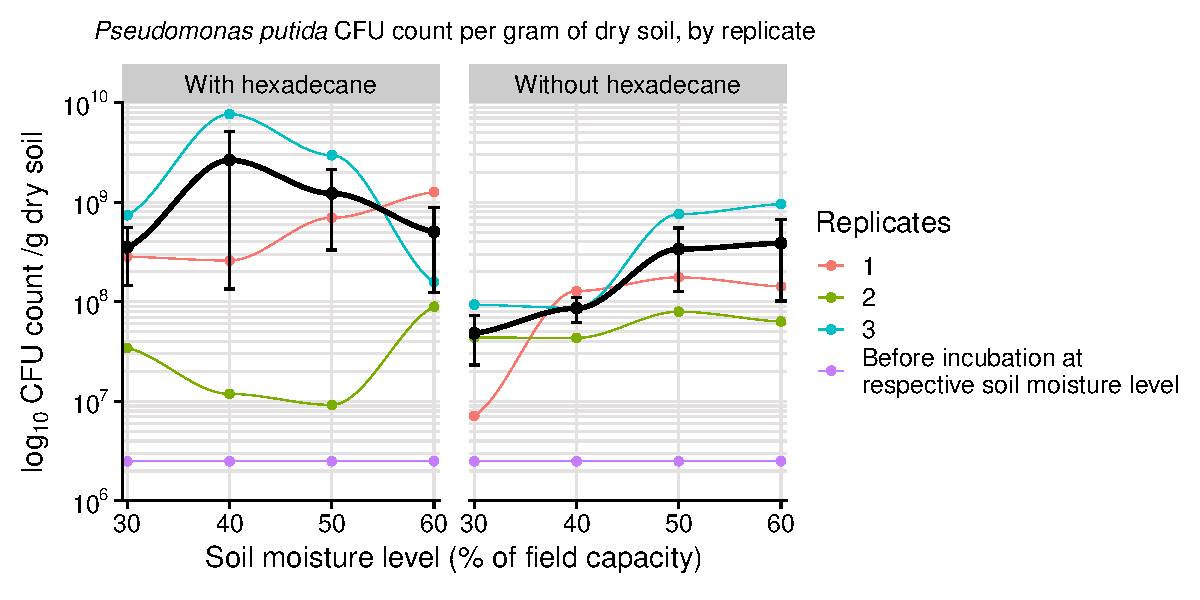
\includegraphics{analysis_files/figure-latex/visualise-allgroups-1.pdf}

\section{Statistical analysis and visualisation of data from spot
replicates}\label{statistical-analysis-and-visualisation-of-data-from-spot-replicates}

\subsection{Read in group 3 data from Excel
file}\label{read-in-group-3-data-from-excel-file}

\begin{Shaded}
\begin{Highlighting}[]
\NormalTok{group3 }\OtherTok{\textless{}{-}} \FunctionTok{read\_excel}\NormalTok{(}\StringTok{\textquotesingle{}data/cfu\_per\_g\_d\_soil\_group3.xlsx\textquotesingle{}}\NormalTok{)}
\end{Highlighting}
\end{Shaded}

\subsection{Convert relevant columns to factors for
analysis}\label{convert-relevant-columns-to-factors-for-analysis}

\begin{Shaded}
\begin{Highlighting}[]
\CommentTok{\# Convert relevant columns to factors for analysis}
\NormalTok{group3}\SpecialCharTok{$}\NormalTok{Plate }\OtherTok{\textless{}{-}} \FunctionTok{as.factor}\NormalTok{(group3}\SpecialCharTok{$}\NormalTok{Plate)}
\NormalTok{group3}\SpecialCharTok{$}\NormalTok{Contamination }\OtherTok{\textless{}{-}} \FunctionTok{as.factor}\NormalTok{(group3}\SpecialCharTok{$}\NormalTok{Contamination)}
\NormalTok{group3}\SpecialCharTok{$}\NormalTok{spot }\OtherTok{\textless{}{-}} \FunctionTok{as.factor}\NormalTok{(group3}\SpecialCharTok{$}\NormalTok{spot)}
\end{Highlighting}
\end{Shaded}

\subsection{Summarise data}\label{summarise-data-1}

Calculate means, standard deviation, sample size and standard error

\begin{Shaded}
\begin{Highlighting}[]
\NormalTok{data\_summary2 }\OtherTok{\textless{}{-}}\NormalTok{ group3 }\SpecialCharTok{\%\textgreater{}\%}
  \FunctionTok{group\_by}\NormalTok{(Plate, Contamination) }\SpecialCharTok{\%\textgreater{}\%}
  \FunctionTok{summarise}\NormalTok{(}\AttributeTok{mean2 =} \FunctionTok{mean}\NormalTok{(cfu\_count),}
            \AttributeTok{sd2 =} \FunctionTok{sd}\NormalTok{(cfu\_count),}
            \AttributeTok{n2 =} \FunctionTok{n}\NormalTok{(),}
            \AttributeTok{se2 =}\NormalTok{ sd2 }\SpecialCharTok{/} \FunctionTok{sqrt}\NormalTok{(n2))}
\end{Highlighting}
\end{Shaded}

\begin{verbatim}
## `summarise()` has grouped output by 'Plate'. You can override using the
## `.groups` argument.
\end{verbatim}

\subsection{Statistical tests}\label{statistical-tests-1}

\subsubsection{Fit a linear model on CFU count by moisture level and
contamination
status}\label{fit-a-linear-model-on-cfu-count-by-moisture-level-and-contamination-status-1}

\begin{Shaded}
\begin{Highlighting}[]
\NormalTok{mod2 }\OtherTok{\textless{}{-}} \FunctionTok{lm}\NormalTok{(cfu\_count }\SpecialCharTok{\textasciitilde{}}\NormalTok{ Plate }\SpecialCharTok{+}\NormalTok{ Contamination, }\AttributeTok{data =}\NormalTok{ group3)}
\end{Highlighting}
\end{Shaded}

\subsubsection{Use the Freedman-Diaconis rule to determine optimal bin
width for
histogram}\label{use-the-freedman-diaconis-rule-to-determine-optimal-bin-width-for-histogram}

\begin{Shaded}
\begin{Highlighting}[]
\NormalTok{iqr2 }\OtherTok{\textless{}{-}} \FunctionTok{IQR}\NormalTok{(group3}\SpecialCharTok{$}\NormalTok{cfu\_count)}
\NormalTok{n2 }\OtherTok{\textless{}{-}} \FunctionTok{nrow}\NormalTok{(group3)}
\NormalTok{bin\_width2 }\OtherTok{\textless{}{-}} \DecValTok{2} \SpecialCharTok{*}\NormalTok{ iqr2 }\SpecialCharTok{/}\NormalTok{ (n2}\SpecialCharTok{\^{}}\NormalTok{(}\DecValTok{1}\SpecialCharTok{/}\DecValTok{3}\NormalTok{))}
\end{Highlighting}
\end{Shaded}

Bin width = 237686445

\subsubsection{Visualise residual distribution to check normality of
residuals}\label{visualise-residual-distribution-to-check-normality-of-residuals-1}

\begin{Shaded}
\begin{Highlighting}[]
\FunctionTok{ggplot}\NormalTok{(group3, }\FunctionTok{aes}\NormalTok{(}\AttributeTok{x =}\NormalTok{ mod2}\SpecialCharTok{$}\NormalTok{residuals)) }\SpecialCharTok{+}
  \FunctionTok{geom\_histogram}\NormalTok{(}\AttributeTok{binwidth =}\NormalTok{ bin\_width2)}
\end{Highlighting}
\end{Shaded}

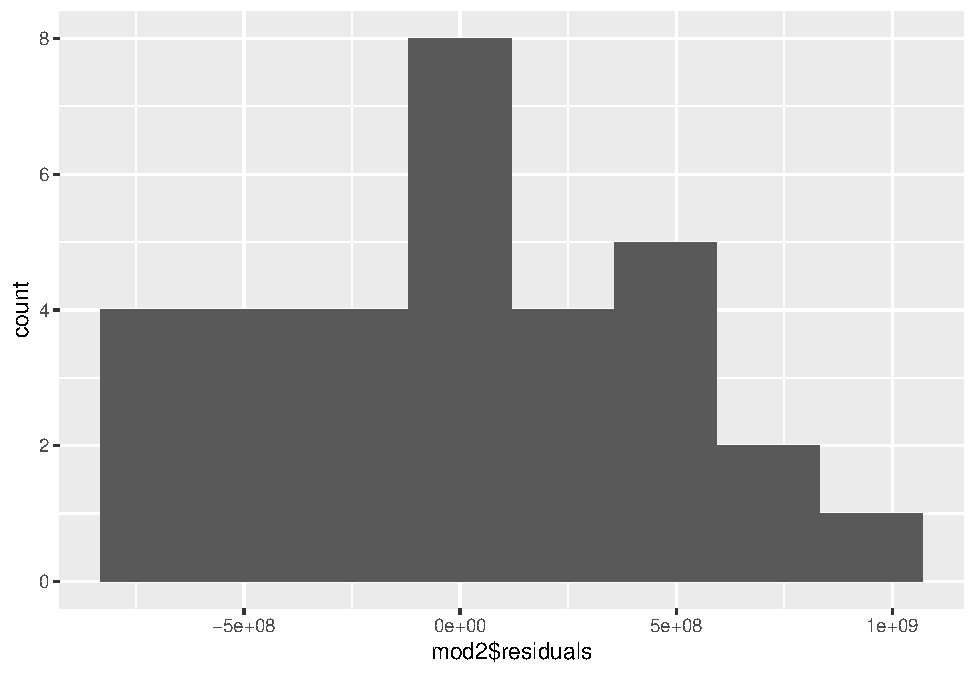
\includegraphics{analysis_files/figure-latex/residuals-group3-1.pdf}

\subsubsection{Shapiro-Wilk test for normality of
residuals}\label{shapiro-wilk-test-for-normality-of-residuals-1}

\begin{Shaded}
\begin{Highlighting}[]
\FunctionTok{shapiro.test}\NormalTok{(mod2}\SpecialCharTok{$}\NormalTok{residuals)}
\end{Highlighting}
\end{Shaded}

\begin{verbatim}
## 
##  Shapiro-Wilk normality test
## 
## data:  mod2$residuals
## W = 0.96822, p-value = 0.4519
\end{verbatim}

p = 0.4519 \textgreater{} 0.05, there is not evidence to suggest that
the data is not normally distributed.

\subsubsection{Levene's test for homogeneity of
variance}\label{levenes-test-for-homogeneity-of-variance-1}

\paragraph{Fit linear model and conduct Levene's
test}\label{fit-linear-model-and-conduct-levenes-test-1}

\begin{Shaded}
\begin{Highlighting}[]
\NormalTok{levmod2 }\OtherTok{\textless{}{-}} \FunctionTok{lm}\NormalTok{(cfu\_count }\SpecialCharTok{\textasciitilde{}}\NormalTok{ Plate }\SpecialCharTok{+}\NormalTok{ Contamination, }\AttributeTok{data =}\NormalTok{ group3)}
\FunctionTok{leveneTest}\NormalTok{(}\FunctionTok{residuals}\NormalTok{(levmod2) }\SpecialCharTok{\textasciitilde{}}\NormalTok{ group3}\SpecialCharTok{$}\NormalTok{spot)}
\end{Highlighting}
\end{Shaded}

\begin{verbatim}
## Levene's Test for Homogeneity of Variance (center = median)
##       Df F value Pr(>F)
## group  3  0.0223 0.9954
##       28
\end{verbatim}

p = 0.9954 \textgreater{} 0.05, therefore there is not enough evidence
to suggest that the data is not homogeneously distributed.

\subsubsection{Plot boxplot of residuals grouped by spot to visualise
the spread of
variance}\label{plot-boxplot-of-residuals-grouped-by-spot-to-visualise-the-spread-of-variance}

\begin{Shaded}
\begin{Highlighting}[]
\NormalTok{group3}\SpecialCharTok{$}\NormalTok{resid }\OtherTok{\textless{}{-}} \FunctionTok{residuals}\NormalTok{(levmod2)}
\FunctionTok{ggplot}\NormalTok{(group3, }\FunctionTok{aes}\NormalTok{(}\AttributeTok{x =}\NormalTok{ spot, }\AttributeTok{y =}\NormalTok{ resid)) }\SpecialCharTok{+}
  \FunctionTok{geom\_boxplot}\NormalTok{() }\SpecialCharTok{+}
  \FunctionTok{labs}\NormalTok{(}\AttributeTok{title =} \StringTok{"Residual Variance by Spot"}\NormalTok{)}
\end{Highlighting}
\end{Shaded}

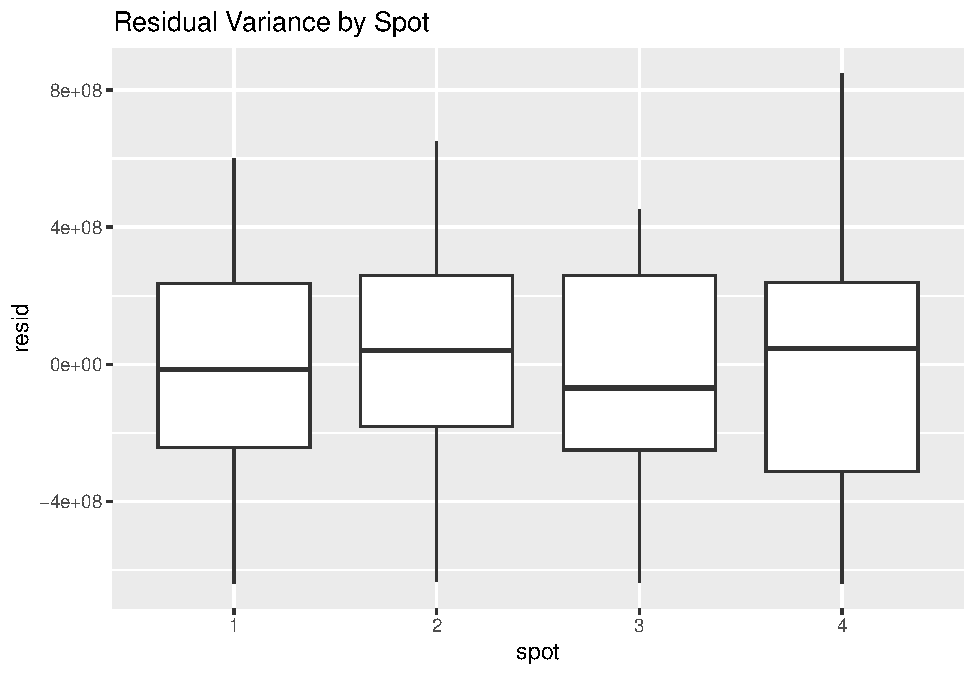
\includegraphics{analysis_files/figure-latex/plot-residuals-group3-1.pdf}

\subsection{Testing for differences in mean CFU count between soil
moisture levels and contamination
status}\label{testing-for-differences-in-mean-cfu-count-between-soil-moisture-levels-and-contamination-status-1}

\subsubsection{We will perform a non-parametric test, eg. the
Scheirer-Ray-Hare test, to observe overall
significance}\label{we-will-perform-a-non-parametric-test-eg.-the-scheirer-ray-hare-test-to-observe-overall-significance-1}

\begin{Shaded}
\begin{Highlighting}[]
\FunctionTok{scheirerRayHare}\NormalTok{(cfu\_count }\SpecialCharTok{\textasciitilde{}}\NormalTok{ Plate }\SpecialCharTok{*}\NormalTok{ Contamination, }\AttributeTok{data =}\NormalTok{ group3)}
\end{Highlighting}
\end{Shaded}

\begin{verbatim}
## 
## DV:  cfu_count 
## Observations:  32 
## D:  0.9998167 
## MS total:  88
\end{verbatim}

\begin{verbatim}
##                     Df  Sum Sq       H  p.value
## Plate                3  336.25  3.8217 0.281369
## Contamination        1  903.12 10.2647 0.001356
## Plate:Contamination  3 1328.13 15.0951 0.001737
## Residuals           24  160.00
\end{verbatim}

p(Plate:Contamination) = 0.001737 \textless{} 0.05, therefore there is
evidence to suggest that soil moisture content does affect growth of P.
putida.

\subsubsection{Post-hoc pairwise
testing}\label{post-hoc-pairwise-testing-1}

\paragraph{Post-hoc for
Contamination}\label{post-hoc-for-contamination-1}

\paragraph{}\label{section-3}

\begin{Shaded}
\begin{Highlighting}[]
\FunctionTok{dunnTest}\NormalTok{(cfu\_count }\SpecialCharTok{\textasciitilde{}}\NormalTok{ Contamination, }\AttributeTok{data =}\NormalTok{ group3, }\AttributeTok{method =} \StringTok{"bonferroni"}\NormalTok{)}
\end{Highlighting}
\end{Shaded}

\begin{verbatim}
## Dunn (1964) Kruskal-Wallis multiple comparison
\end{verbatim}

\begin{verbatim}
##   p-values adjusted with the Bonferroni method.
\end{verbatim}

\begin{verbatim}
##                             Comparison        Z     P.unadj       P.adj
## 1 With hexadecane - Without hexadecane 3.203852 0.001356023 0.001356023
\end{verbatim}

p.adj = 0.001356023 \textless{} 0.05, therefore there is evidence to
suggest that hexadecane presence does affect growth of P. putida.

\paragraph{Post-hoc for Plate}\label{post-hoc-for-plate-1}

\subparagraph{Contamination = With
hexadecane}\label{contamination-with-hexadecane-1}

\subparagraph{}\label{section-4}

\begin{Shaded}
\begin{Highlighting}[]
\FunctionTok{dunnTest}\NormalTok{(cfu\_count }\SpecialCharTok{\textasciitilde{}}\NormalTok{ Plate, }\AttributeTok{data =} \FunctionTok{filter}\NormalTok{(group3, Contamination }\SpecialCharTok{==} \StringTok{"With hexadecane"}\NormalTok{), }\AttributeTok{method =} \StringTok{"bh"}\NormalTok{)}
\end{Highlighting}
\end{Shaded}

\begin{verbatim}
## Dunn (1964) Kruskal-Wallis multiple comparison
\end{verbatim}

\begin{verbatim}
##   p-values adjusted with the Benjamini-Hochberg method.
\end{verbatim}

\begin{verbatim}
##   Comparison         Z      P.unadj       P.adj
## 1    30 - 40 -2.376354 0.0174846744 0.034969349
## 2    30 - 50 -1.188177 0.2347636628 0.234763663
## 3    40 - 50  1.188177 0.2347636628 0.281716395
## 4    30 - 60  1.188177 0.2347636628 0.352145494
## 5    40 - 60  3.564531 0.0003645072 0.002187043
## 6    50 - 60  2.376354 0.0174846744 0.052454023
\end{verbatim}

\subparagraph{Contamination = Without
hexadecane}\label{contamination-without-hexadecane-1}

\subparagraph{}\label{section-5}

\begin{Shaded}
\begin{Highlighting}[]
\FunctionTok{dunnTest}\NormalTok{(cfu\_count }\SpecialCharTok{\textasciitilde{}}\NormalTok{ Plate, }\AttributeTok{data =} \FunctionTok{filter}\NormalTok{(group3, Contamination }\SpecialCharTok{==} \StringTok{"Without hexadecane"}\NormalTok{), }\AttributeTok{method =} \StringTok{"bh"}\NormalTok{)}
\end{Highlighting}
\end{Shaded}

\begin{verbatim}
## Dunn (1964) Kruskal-Wallis multiple comparison
\end{verbatim}

\begin{verbatim}
##   p-values adjusted with the Benjamini-Hochberg method.
\end{verbatim}

\begin{verbatim}
##   Comparison          Z     P.unadj      P.adj
## 1    30 - 40  0.2972629 0.766265789 0.76626579
## 2    30 - 50 -1.8578932 0.063184176 0.09477626
## 3    40 - 50 -2.1551562 0.031149616 0.06229923
## 4    30 - 60 -2.6010505 0.009293876 0.02788163
## 5    40 - 60 -2.8983135 0.003751754 0.02251052
## 6    50 - 60 -0.7431573 0.457386453 0.54886374
\end{verbatim}

With hexadecane: Only significant difference between 30-40\% and
40-60\%, p.adj = 0.034969349 and 0.002187043, respectively. Without
hexadecane: Only significant difference between 30-60\% and 40-60\%,
p.adj = 0.02788163 and 0.02251052, respectively. Therefore there is
evidence to suggest that soil moisture content does affect the growth of
P. putida, using data from group 3. However, as p.adj (With hexadecane,
30-40\%) \textgreater{} 0.025 and the difference is positive, we cannot
conclude that the difference between 30\% and 40\% is significant with a
one-tailed test. The same is true for p.adj (Without hexadecane,
30-60\%).

\subsection{Visualise group 3 CFU count with group means, SE, smoothed
lines, and statistical
annotations}\label{visualise-group-3-cfu-count-with-group-means-se-smoothed-lines-and-statistical-annotations}

\subsubsection{Preparing statistical
annotations.}\label{preparing-statistical-annotations.}

\begin{Shaded}
\begin{Highlighting}[]
\NormalTok{pairwise\_p }\OtherTok{\textless{}{-}} \FunctionTok{data.frame}\NormalTok{(}
  \AttributeTok{group1 =} \FunctionTok{c}\NormalTok{(}\StringTok{"30"}\NormalTok{, }\StringTok{"40"}\NormalTok{, }\StringTok{"30"}\NormalTok{, }\StringTok{"40"}\NormalTok{),}
  \AttributeTok{group2 =} \FunctionTok{c}\NormalTok{(}\StringTok{"40"}\NormalTok{, }\StringTok{"60"}\NormalTok{, }\StringTok{"60"}\NormalTok{, }\StringTok{"60"}\NormalTok{),}
  \AttributeTok{y.position =} \FunctionTok{c}\NormalTok{(}\FloatTok{2.05e9}\NormalTok{, }\FloatTok{2.10e9}\NormalTok{, }\DecValTok{300000000}\NormalTok{, }\DecValTok{500000000}\NormalTok{),}
  \AttributeTok{p.adj =} \FunctionTok{c}\NormalTok{(}\FloatTok{0.034969349}\NormalTok{, }\FloatTok{0.002187043}\NormalTok{, }\FloatTok{0.02788163}\NormalTok{, }\FloatTok{0.02251052}\NormalTok{),}
  \AttributeTok{Contamination =} \FunctionTok{c}\NormalTok{(}\StringTok{"With hexadecane"}\NormalTok{, }\StringTok{"With hexadecane"}\NormalTok{, }
                    \StringTok{"Without hexadecane"}\NormalTok{, }\StringTok{"Without hexadecane"}\NormalTok{)}
\NormalTok{)}

\NormalTok{pairwise\_p}\SpecialCharTok{$}\NormalTok{label }\OtherTok{\textless{}{-}} \FunctionTok{paste0}\NormalTok{(}\StringTok{"p.adj = "}\NormalTok{, }\FunctionTok{signif}\NormalTok{(pairwise\_p}\SpecialCharTok{$}\NormalTok{p.adj, }\DecValTok{3}\NormalTok{))}
\end{Highlighting}
\end{Shaded}

\subsubsection{Create plot}\label{create-plot-1}

\begin{Shaded}
\begin{Highlighting}[]
\NormalTok{mean\_CFU\_count2 }\OtherTok{\textless{}{-}} \FunctionTok{ggplot}\NormalTok{() }\SpecialCharTok{+}
  
  \DocumentationTok{\#\#\#\# Plotting data points.}
  \FunctionTok{geom\_point}\NormalTok{(}\AttributeTok{data =}\NormalTok{ group3,}
             \FunctionTok{aes}\NormalTok{(}\AttributeTok{x =} \FunctionTok{factor}\NormalTok{(Plate), }
                 \AttributeTok{y =}\NormalTok{ cfu\_count, }
                 \AttributeTok{colour =}\NormalTok{ Contamination)) }\SpecialCharTok{+}
  
  \DocumentationTok{\#\#\#\# Plotting LOESS regression lines from data\_tidy.}
  \FunctionTok{geom\_smooth}\NormalTok{(}\AttributeTok{data =}\NormalTok{ group3,}
              \FunctionTok{aes}\NormalTok{(}\AttributeTok{x =} \FunctionTok{factor}\NormalTok{(Plate), }
                  \AttributeTok{y =}\NormalTok{ cfu\_count, }
                  \AttributeTok{colour =}\NormalTok{ Contamination), }
              \AttributeTok{method =} \StringTok{"loess"}\NormalTok{, }
              \AttributeTok{se =} \ConstantTok{FALSE}\NormalTok{,}
              \AttributeTok{linewidth =} \FloatTok{0.3}\NormalTok{) }\SpecialCharTok{+}
  
  \DocumentationTok{\#\#\#\# Plotting means from data\_summary.}
  \FunctionTok{geom\_point}\NormalTok{(}\AttributeTok{data =}\NormalTok{ data\_summary2, }
             \FunctionTok{aes}\NormalTok{(}\AttributeTok{x =} \FunctionTok{factor}\NormalTok{(Plate), }
                 \AttributeTok{y =}\NormalTok{ mean2), }
             \AttributeTok{colour =} \StringTok{\textquotesingle{}black\textquotesingle{}}\NormalTok{, }
             \AttributeTok{size =} \DecValTok{2}\NormalTok{) }\SpecialCharTok{+}
  
  \DocumentationTok{\#\#\#\# Plotting error bars for means from data\_summary.}
  \FunctionTok{geom\_errorbar}\NormalTok{(}\AttributeTok{data =}\NormalTok{ data\_summary2,}
                \FunctionTok{aes}\NormalTok{(}\AttributeTok{x =} \FunctionTok{factor}\NormalTok{(Plate), }
                    \AttributeTok{ymin =}\NormalTok{ mean2 }\SpecialCharTok{{-}}\NormalTok{ se2, }
                    \AttributeTok{ymax =}\NormalTok{ mean2 }\SpecialCharTok{+}\NormalTok{ se2), }
                \AttributeTok{width =} \FloatTok{0.1}\NormalTok{, }
                \AttributeTok{colour =} \StringTok{"black"}\NormalTok{) }\SpecialCharTok{+}
  
  \DocumentationTok{\#\#\#\# Plotting LOESS regression lines for the means.}
  \FunctionTok{geom\_smooth}\NormalTok{(}\AttributeTok{data =}\NormalTok{ data\_summary2,}
              \FunctionTok{aes}\NormalTok{(}\AttributeTok{x =} \FunctionTok{factor}\NormalTok{(Plate), }
                  \AttributeTok{y =}\NormalTok{ mean2,}
                  \AttributeTok{group =}\NormalTok{ Contamination), }
              \AttributeTok{method =} \StringTok{"loess"}\NormalTok{, }
              \AttributeTok{colour =} \StringTok{"black"}\NormalTok{,}
              \AttributeTok{se =} \ConstantTok{FALSE}\NormalTok{, }
              \AttributeTok{linewidth =} \DecValTok{1}\NormalTok{) }\SpecialCharTok{+}
  
  \DocumentationTok{\#\#\#\# Adding labels and changing axis.}
  \FunctionTok{labs}\NormalTok{(}\AttributeTok{title =} \FunctionTok{expression}\NormalTok{(}\FunctionTok{italic}\NormalTok{(}\StringTok{"Pseudomonas putida"}\NormalTok{)}\SpecialCharTok{\textasciitilde{}}\StringTok{"}\SpecialCharTok{\textbackslash{}n}\StringTok{CFU count per gram of dry soil"}\NormalTok{),}
       \AttributeTok{x =} \FunctionTok{expression}\NormalTok{(}\StringTok{"Soil moisture level /\% of field capacity"}\NormalTok{),}
       \AttributeTok{y =} \FunctionTok{expression}\NormalTok{(}\StringTok{"CFU count /g dry soil"}\NormalTok{),}
       \AttributeTok{colour =} \StringTok{"Contamination"}\NormalTok{) }\SpecialCharTok{+}
  
  \DocumentationTok{\#\#\#\# Adjusting the axes and legend.}
  \FunctionTok{scale\_x\_discrete}\NormalTok{(}\AttributeTok{labels =} \FunctionTok{c}\NormalTok{(}\StringTok{"30"}\NormalTok{, }\StringTok{"40"}\NormalTok{, }\StringTok{"50"}\NormalTok{, }\StringTok{"60"}\NormalTok{),}
                   \AttributeTok{expand =} \FunctionTok{c}\NormalTok{(}\DecValTok{0}\NormalTok{, }\DecValTok{0}\NormalTok{)}
\NormalTok{  ) }\SpecialCharTok{+}
  \FunctionTok{scale\_y\_continuous}\NormalTok{(}
    \AttributeTok{labels =} \ControlFlowTok{function}\NormalTok{(x) \{}
      \FunctionTok{sapply}\NormalTok{(x, }\ControlFlowTok{function}\NormalTok{(val) \{}
        \ControlFlowTok{if}\NormalTok{ (val }\SpecialCharTok{==} \DecValTok{0}\NormalTok{) \{}
          \StringTok{"0"}
\NormalTok{        \} }\ControlFlowTok{else}\NormalTok{ \{}
\NormalTok{          formatted }\OtherTok{\textless{}{-}} \FunctionTok{formatC}\NormalTok{(val }\SpecialCharTok{/} \DecValTok{10}\SpecialCharTok{\^{}}\FunctionTok{floor}\NormalTok{(}\FunctionTok{log10}\NormalTok{(val)), }\AttributeTok{digits =} \DecValTok{2}\NormalTok{, }\AttributeTok{format =} \StringTok{"f"}\NormalTok{)}
\NormalTok{          exponent }\OtherTok{\textless{}{-}} \FunctionTok{floor}\NormalTok{(}\FunctionTok{log10}\NormalTok{(val))}
          \FunctionTok{parse}\NormalTok{(}\AttributeTok{text =} \FunctionTok{paste0}\NormalTok{(formatted, }\StringTok{" \%*\% 10\^{}"}\NormalTok{, exponent))}
\NormalTok{        \}}
\NormalTok{      \})}
\NormalTok{    \},}
    \AttributeTok{breaks =} \FunctionTok{seq}\NormalTok{(}\DecValTok{0}\NormalTok{, }\FloatTok{2.25e9}\NormalTok{, }\AttributeTok{by =} \FloatTok{2.5e8}\NormalTok{),}
    \AttributeTok{limits =} \FunctionTok{c}\NormalTok{(}\DecValTok{0}\NormalTok{, }\FloatTok{2.25e9}\NormalTok{),}
    \AttributeTok{expand =} \FunctionTok{c}\NormalTok{(}\DecValTok{0}\NormalTok{, }\DecValTok{0}\NormalTok{)}
\NormalTok{  ) }\SpecialCharTok{+}
  \FunctionTok{scale\_colour\_manual}\NormalTok{(}\AttributeTok{values =} \FunctionTok{c}\NormalTok{(}\StringTok{\textquotesingle{}With hexadecane\textquotesingle{}} \OtherTok{=} \StringTok{\textquotesingle{}\#F8766D\textquotesingle{}}\NormalTok{, }\StringTok{\textquotesingle{}Without hexadecane\textquotesingle{}} \OtherTok{=} \StringTok{\textquotesingle{}\#00BFC4\textquotesingle{}}\NormalTok{, }\StringTok{\textquotesingle{}4\textquotesingle{}} \OtherTok{=} \StringTok{\textquotesingle{}\#C77CFF\textquotesingle{}}\NormalTok{),}
                      \AttributeTok{labels =} \FunctionTok{c}\NormalTok{(}\StringTok{\textquotesingle{}With hexadecane\textquotesingle{}}\NormalTok{, }\StringTok{\textquotesingle{}Without hexadecane\textquotesingle{}}\NormalTok{, }
                                 \StringTok{\textquotesingle{}Before incubation at }\SpecialCharTok{\textbackslash{}n}\StringTok{respective soil moisture level\textquotesingle{}}\NormalTok{)) }\SpecialCharTok{+}
  \FunctionTok{geom\_point}\NormalTok{(}\AttributeTok{data =}\NormalTok{ group3,}
             \FunctionTok{aes}\NormalTok{(}\AttributeTok{x =} \FunctionTok{factor}\NormalTok{(Plate), }
                 \AttributeTok{y =}\NormalTok{ cfu\_count, }
                 \AttributeTok{colour =}\NormalTok{ Contamination)) }\SpecialCharTok{+}
  
  \DocumentationTok{\#\#\#\# Adding statistical annotations.}
  \FunctionTok{stat\_pvalue\_manual}\NormalTok{(pairwise\_p, }
                     \AttributeTok{label =} \StringTok{"label"}\NormalTok{, }
                     \AttributeTok{xmin =} \StringTok{"group1"}\NormalTok{, }\AttributeTok{xmax =} \StringTok{"group2"}\NormalTok{, }
                     \AttributeTok{y.position =} \StringTok{"y.position"}\NormalTok{, }
                     \AttributeTok{tip.length =} \FloatTok{0.01}\NormalTok{,}
                     \AttributeTok{size =} \DecValTok{3}\NormalTok{,}
                     \AttributeTok{bracket.size =} \FloatTok{0.3}\NormalTok{) }\SpecialCharTok{+}
  
  \DocumentationTok{\#\#\#\# Theming.}
\NormalTok{  cowplot}\SpecialCharTok{::}\FunctionTok{theme\_cowplot}\NormalTok{() }\SpecialCharTok{+}
\NormalTok{  theme\_custom }\SpecialCharTok{+}
\FunctionTok{theme}\NormalTok{(}\AttributeTok{axis.text.x =} \FunctionTok{element\_text}\NormalTok{(}\AttributeTok{angle =} \DecValTok{0}\NormalTok{, }\AttributeTok{hjust =} \DecValTok{1}\NormalTok{))}

\NormalTok{mean\_CFU\_count2}
\end{Highlighting}
\end{Shaded}

\begin{verbatim}
## `geom_smooth()` using formula = 'y ~ x'
## `geom_smooth()` using formula = 'y ~ x'
\end{verbatim}

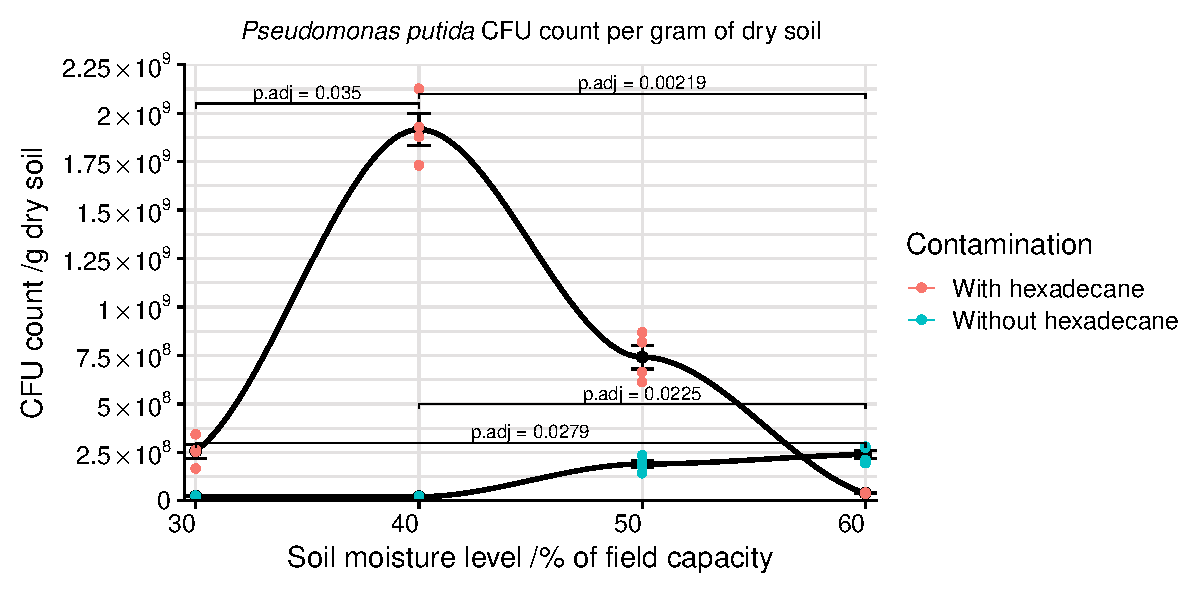
\includegraphics{analysis_files/figure-latex/visualise-group3-1.pdf}

\subsection{References}\label{references}

\begin{Shaded}
\begin{Highlighting}[]
\NormalTok{Dunn, O.J. (1964) \textquotesingle{}Multiple comparisons using rank sums\textquotesingle{}, *Technometrics*, 6(3), pp. 241–252.  }
\NormalTok{Fox, J. and Weisberg, S. (2019) *An R Companion to Applied Regression*. 3rd edn. Thousand Oaks, CA: Sage.  }
\NormalTok{Kassambara, A. (2023) *ggpubr: \textquotesingle{}ggplot2\textquotesingle{}{-}Based Publication Ready Plots*. R package version 0.6.0.  }
\NormalTok{Levene, H., 1960. **Robust tests for equality of variances*. In: I. Olkin, ed. 1960. Contributions to probability and statistics: essays in honor of Harold Hotelling. Stanford: Stanford University Press, pp.278–292.}
\NormalTok{Mangiafico, S. (2024) *rcompanion: Functions to Support Extension Education Program Evaluation*. R package version 2.4.30.  }
\NormalTok{Ogle, D.H. et al. (2024) *FSA: Fisheries Stock Analysis*. R package version 0.9.5.  }
\NormalTok{Oksanen, J. et al. (2022) *vegan: Community Ecology Package*. R package version 2.6{-}4.  }
\NormalTok{R Core Team (2024) *R: A Language and Environment for Statistical Computing*. Vienna: R Foundation for Statistical Computing.  }
\NormalTok{Scheirer, C.J., Ray, W.S. and Hare, N. (1976) \textquotesingle{}The analysis of ranked data derived from completely randomized factorial designs\textquotesingle{}, *Biometrics*, 32(2), pp. 429–434.  }
\NormalTok{Shapiro, S.S. and Wilk, M.B. (1965) \textquotesingle{}An analysis of variance test for normality (complete samples)\textquotesingle{}, *Biometrika*, 52(3/4), pp. 591–611.   }
\NormalTok{Wickham, H. (2016) *ggplot2: Elegant Graphics for Data Analysis*. New York: Springer.  }
\NormalTok{Wickham, H. et al. (2019) *Welcome to the tidyverse*. R package version 2.0.0.  }
\NormalTok{Wickham, H. and Bryan, J. (2023) *readxl: Read Excel Files*. R package version 1.4.3.  }
\NormalTok{Wickham, H. and Seidel, D. (2022) *scales: Scale Functions for Visualization*. R package version 1.3.0.}
\end{Highlighting}
\end{Shaded}


\end{document}
